%==============================================================================
%  INFORME: SOLUCIÓN NUMÉRICA DE ECUACIONES DE POISSON Y LAPLACE
%  Compilar en Overleaf (pdflatex)
%==============================================================================
\documentclass[12pt, a4paper]{article}

%--- Idioma y codificación ---
\usepackage[spanish]{babel}
\usepackage[utf8]{inputenc}
\usepackage[T1]{fontenc}

%--- Matemáticas ---
\usepackage{amsmath, amssymb, mathtools}

%--- Diseño de página ---
\usepackage[top=2.5cm, bottom=2.5cm, left=2.8cm, right=2.8cm]{geometry}
\usepackage{setspace}
\onehalfspacing

%--- Gráficos y figuras ---
\usepackage{graphicx}
\usepackage{caption}
\usepackage{subcaption}
\usepackage{float}

%--- Tablas ---
\usepackage{booktabs}
\usepackage{array}
\usepackage{multirow}

%--- Código fuente ---
\usepackage{listings}
\usepackage{xcolor}

%--- Hipervínculos ---
\usepackage{hyperref}
\hypersetup{
    colorlinks=true,
    linkcolor=blue!60!black,
    citecolor=green!50!black,
    urlcolor=blue!70!black
}

%--- Otros ---
\usepackage{parskip}
\usepackage{enumitem}
\usepackage{fancyhdr}
\usepackage{titlesec}

%==============================================================================
%  CONFIGURACIÓN DE LISTINGS (código fuente)
%==============================================================================
\definecolor{codebg}{RGB}{245,245,245}
\definecolor{codeframe}{RGB}{180,180,180}
\definecolor{keyword}{RGB}{0,0,180}
\definecolor{comment}{RGB}{0,130,0}
\definecolor{string}{RGB}{160,0,0}

\lstdefinestyle{fortranstyle}{
  language=Fortran,
  backgroundcolor=\color{codebg},
  frame=single, framerule=0.5pt, rulecolor=\color{codeframe},
  basicstyle=\ttfamily\small,
  keywordstyle=\color{keyword}\bfseries,
  commentstyle=\color{comment}\itshape,
  stringstyle=\color{string},
  numbers=left, numberstyle=\tiny\color{gray}, numbersep=6pt,
  breaklines=true, breakatwhitespace=true,
  tabsize=2, showstringspaces=false,
  morekeywords={real,allocatable,intent,implicit,none,deallocate,allocate,
                do,end,if,then,exit,write,call,subroutine,program,parameter}
}

\lstdefinestyle{cppstyle}{
  language=C++,
  backgroundcolor=\color{codebg},
  frame=single, framerule=0.5pt, rulecolor=\color{codeframe},
  basicstyle=\ttfamily\small,
  keywordstyle=\color{keyword}\bfseries,
  commentstyle=\color{comment}\itshape,
  stringstyle=\color{string},
  numbers=left, numberstyle=\tiny\color{gray}, numbersep=6pt,
  breaklines=true, breakatwhitespace=true,
  tabsize=2, showstringspaces=false,
}

\lstdefinestyle{pythonstyle}{
  language=Python,
  backgroundcolor=\color{codebg},
  frame=single, framerule=0.5pt, rulecolor=\color{codeframe},
  basicstyle=\ttfamily\small,
  keywordstyle=\color{keyword}\bfseries,
  commentstyle=\color{comment}\itshape,
  stringstyle=\color{string},
  numbers=left, numberstyle=\tiny\color{gray}, numbersep=6pt,
  breaklines=true, breakatwhitespace=true,
  tabsize=4, showstringspaces=false,
}

%==============================================================================
%  ENCABEZADO Y PIE DE PÁGINA
%==============================================================================
\pagestyle{fancy}
\fancyhf{}
\fancyhead[L]{\small Modelamiento FC — Taller: Ecuaciones de Poisson y Laplace}
\fancyhead[R]{\small \thepage}
\renewcommand{\headrulewidth}{0.4pt}

%==============================================================================
%  DOCUMENTO
%==============================================================================
\begin{document}

%--- PORTADA ---
\begin{titlepage}
  \centering
  \vspace*{1.5cm}

  {\Large \textbf{Modelamiento en Física Computacional}}\\[0.4cm]
  {\large Taller Práctico}\\[2cm]

  \rule{\linewidth}{1pt}\\[0.4cm]
  {\LARGE \textbf{Solución Numérica de Ecuaciones de}}\\[0.3cm]
  {\LARGE \textbf{Poisson y Laplace}}\\[0.3cm]
  {\large Método de Diferencias Finitas con Iteración de Jacobi}\\[0.3cm]
  \rule{\linewidth}{1pt}\\[1.5cm]

  {\large \textbf{Comparativa de Rendimiento: Fortran, C++ y Python}}\\[2cm]

  \begin{tabular}{ll}
    \textbf{Método numérico:} & Diferencias Finitas Centradas (orden 2) \\[0.2cm]
    \textbf{Iteración:}       & Jacobi \\[0.2cm]
    \textbf{Mallas evaluadas:} & $100\times100$ y $500\times500$ \\[0.2cm]
    \textbf{Tolerancia:}      & $10^{-6}$ \\[0.2cm]
    \textbf{Iteraciones máx.:} & $400\,000$ \\[0.2cm]
    \textbf{Precisión:}       & Doble precisión (64-bit float) \\
  \end{tabular}

  \vfill
  {\large Marzo 2026}
\end{titlepage}

%--- TABLA DE CONTENIDOS ---
\tableofcontents
\newpage

%==============================================================================
\section{Introducción}
%==============================================================================

Las ecuaciones de Poisson y Laplace son EDP elípticas fundamentales en
física computacional, con aplicaciones en electrostática, conducción de calor,
flujo potencial e ingeniería estructural. Su forma general en dos dimensiones es:

\begin{equation}
  \nabla^2 V = \frac{\partial^2 V}{\partial x^2} + \frac{\partial^2 V}{\partial y^2} = f(x,y)
  \label{eq:poisson_general}
\end{equation}

donde $f=0$ corresponde a la ecuación de Laplace y $f\neq 0$ a la de Poisson.

En este taller se implementa el método de diferencias finitas (FDM) con
iteración de Jacobi para resolver cuatro problemas con solución analítica
conocida, lo que permite verificar la exactitud del método. Se comparan tres
implementaciones equivalentes en \textbf{Fortran}, \textbf{C++} y
\textbf{Python (numpy)} sobre mallas de $100\times100$ y $500\times500$ nodos,
cuantificando las diferencias de rendimiento computacional entre lenguajes
compilados y un entorno vectorizado interpretado.

%==============================================================================
\section{Descripción de los Problemas Físicos}
%==============================================================================

Se resuelven cuatro ecuaciones sobre dominios rectangulares 2D, todas con
solución analítica conocida que sirve para verificar el error del método
numérico.

%------------------------------------------------------------------------------
\subsection{Ejercicio 1 — Poisson: fuente exponencial}
%------------------------------------------------------------------------------

\begin{equation}
  \nabla^2 V = (x^2 + y^2)\,e^{xy}, \qquad (x,y)\in[0,2]\times[0,1]
  \label{eq:ej1}
\end{equation}

\textbf{Condiciones de contorno:}
\[
  V(0,y)=1,\quad V(2,y)=e^{2y},\quad V(x,0)=1,\quad V(x,1)=e^x
\]

\textbf{Solución analítica:} $V(x,y) = e^{xy}$

%------------------------------------------------------------------------------
\subsection{Ejercicio 2 — Laplace}
%------------------------------------------------------------------------------

\begin{equation}
  \nabla^2 V = 0, \qquad (x,y)\in[1,2]\times[0,1]
  \label{eq:ej2}
\end{equation}

\textbf{Condiciones de contorno:}
\[
  V(1,y)=\ln(y^2+1),\quad V(2,y)=\ln(y^2+4),\quad
  V(x,0)=2\ln x,\quad V(x,1)=\ln(x^2+1)
\]

\textbf{Solución analítica:} $V(x,y) = \ln(x^2+y^2)$

%------------------------------------------------------------------------------
\subsection{Ejercicio 3 — Poisson: fuente constante}
%------------------------------------------------------------------------------

\begin{equation}
  \nabla^2 V = 4, \qquad (x,y)\in[1,2]\times[0,2]
  \label{eq:ej3}
\end{equation}

\textbf{Condiciones de contorno:} consistentes con $V(x,y)=(x-y)^2$:
\[
  V(1,y)=(1-y)^2,\quad V(2,y)=(2-y)^2,\quad V(x,0)=x^2,\quad V(x,2)=(x-2)^2
\]

\textbf{Solución analítica:} $V(x,y) = (x-y)^2$

%------------------------------------------------------------------------------
\subsection{Ejercicio 4 — Poisson: fuente variable}
%------------------------------------------------------------------------------

\begin{equation}
  \nabla^2 V = \frac{x}{y} + \frac{y}{x}, \qquad (x,y)\in[1,2]\times[1,2]
  \label{eq:ej4}
\end{equation}

\textbf{Condiciones de contorno:}
\[
  V(1,y)=y\ln y,\quad V(2,y)=2y\ln(2y),\quad
  V(x,1)=x\ln x,\quad V(x,2)=2x\ln(2x)
\]

\textbf{Solución analítica:} $V(x,y) = xy\ln(xy)$

%==============================================================================
\section{Metodología Numérica}
%==============================================================================

%------------------------------------------------------------------------------
\subsection{Discretización por diferencias finitas centradas}
%------------------------------------------------------------------------------

El dominio $[x_0,x_f]\times[y_0,y_f]$ se discretiza con una malla uniforme de
$(M+1)\times(N+1)$ nodos, con pasos $h=\Delta x=(x_f-x_0)/M$ y
$k=\Delta y=(y_f-y_0)/N$. Aplicando la aproximación de segundo orden para el
laplaciano:

\[
  \frac{\partial^2 V}{\partial x^2}\bigg|_{i,j} \approx
    \frac{V_{i,j+1} - 2V_{i,j} + V_{i,j-1}}{h^2}, \qquad
  \frac{\partial^2 V}{\partial y^2}\bigg|_{i,j} \approx
    \frac{V_{i+1,j} - 2V_{i,j} + V_{i-1,j}}{k^2}
\]

sustituyendo en \eqref{eq:poisson_general} y despejando $V_{i,j}$ se obtiene
la \textbf{ecuación de actualización de 5 puntos}:

\begin{equation}
  \boxed{
  V_{i,j} = \frac{
    \left(V_{i+1,j} + V_{i-1,j}\right)k^2 +
    \left(V_{i,j+1} + V_{i,j-1}\right)h^2 -
    f_{i,j}\,h^2 k^2
  }{2(h^2 + k^2)}
  }
  \label{eq:5puntos}
\end{equation}

donde los índices $i$ y $j$ recorren las filas (dirección $y$) y columnas
(dirección $x$) del interior de la malla, respectivamente.

%------------------------------------------------------------------------------
\subsection{Iteración de Jacobi}
%------------------------------------------------------------------------------

En la iteración de Jacobi, el arreglo completo $V^{(n+1)}$ se calcula
\emph{exclusivamente} a partir de los valores del paso anterior $V^{(n)}$:

\begin{equation}
  V_{i,j}^{(n+1)} = \frac{
    \left(V_{i+1,j}^{(n)} + V_{i-1,j}^{(n)}\right)k^2 +
    \left(V_{i,j+1}^{(n)} + V_{i,j-1}^{(n)}\right)h^2 -
    f_{i,j}\,h^2 k^2
  }{2(h^2 + k^2)}
  \label{eq:jacobi}
\end{equation}

Esta estructura exige mantener dos arreglos en memoria simultáneamente
($V$ y $V_\text{new}$), a diferencia de Gauss-Seidel que actualiza en el lugar.
El criterio de parada es:

\begin{equation}
  \delta^{(n)} = \max_{i,j}\left|V_{i,j}^{(n+1)} - V_{i,j}^{(n)}\right| < 10^{-6}
  \label{eq:criterio}
\end{equation}

\textbf{Parámetros comunes a las tres implementaciones:}

\begin{table}[H]
  \centering
  \begin{tabular}{ll}
    \toprule
    \textbf{Parámetro} & \textbf{Valor} \\
    \midrule
    Tolerancia $\delta$ & $10^{-6}$ \\
    Iteraciones máximas & $400\,000$ \\
    Precisión aritmética & Doble (64-bit, \texttt{real(8)} / \texttt{double}) \\
    Inicialización interior & $V_{i,j}^{(0)} = 0$ \\
    \bottomrule
  \end{tabular}
  \caption{Parámetros comunes a las tres implementaciones.}
  \label{tab:params}
\end{table}

%------------------------------------------------------------------------------
\subsection{Complejidad computacional}
%------------------------------------------------------------------------------

Jacobi en una malla $N\times N$ tiene:
\begin{itemize}[noitemsep]
  \item \textbf{Trabajo por iteración:} $\mathcal{O}(N^2)$ — se recorre todo el interior.
  \item \textbf{Iteraciones hasta convergencia:} $\mathcal{O}(N^2)$, ya que el radio
        espectral satisface $\rho \approx 1 - \tfrac{\pi^2}{2}h^2$ con $h=1/N$,
        por lo que se necesitan $\sim \pi^2/(2h^2) \propto N^2$ iteraciones.
  \item \textbf{Trabajo total:} $\mathcal{O}(N^4)$.
\end{itemize}

%==============================================================================
\section{Implementaciones}
%==============================================================================

%------------------------------------------------------------------------------
\subsection{Fortran (\texttt{poisson\_laplace.f90})}
%------------------------------------------------------------------------------

Compilación: \texttt{gfortran -O2 -o poisson\_laplace poisson\_laplace.f90}

El código emplea arreglos \texttt{allocatable} de doble precisión
(\texttt{real(8)}). El índice $i$ recorre la dirección $y$ y el índice $j$ la
dirección $x$, en concordancia con el almacenamiento column-major de Fortran.
El tiempo se mide con \texttt{cpu\_time()}.

\begin{lstlisting}[style=fortranstyle, caption={Núcleo de Jacobi en Fortran (Ejercicio 1).}]
T_new = T
do it = 1, 400000
  delta = 0.0d0
  do i = 1, N-1
    do j = 1, M-1
      T_new(i,j) = ( (T(i+1,j) + T(i-1,j))*k2   &
                   + (T(i,j+1) + T(i,j-1))*h2    &
                   - source(i,j)*h2*k2            ) / denom
      delta = max(delta, abs(T_new(i,j) - T(i,j)))
    end do
  end do
  T = T_new
  if (delta < tol) then
    write(*,'(A,I6,A)') "  Convergio en ", it, " iteraciones."
    exit
  end if
end do
\end{lstlisting}

%------------------------------------------------------------------------------
\subsection{C++ (\texttt{poisson\_serial.cpp})}
%------------------------------------------------------------------------------

Compilación: \texttt{g++ -O2 -o poisson\_serial poisson\_serial.cpp}

El código usa \texttt{std::vector<std::vector<double>>} para el almacenamiento
2D. El tiempo se mide con \texttt{std::chrono::high\_resolution\_clock}.
Las funciones de condición de contorno y término fuente se seleccionan
mediante un \texttt{switch} sobre una variable global \texttt{case\_selector}.

\begin{lstlisting}[style=cppstyle, caption={Núcleo de Jacobi en C++.}]
static constexpr int    MAX_ITERATIONS = 400000;
static constexpr double TOLERANCE      = 1e-6;

// ...

while (delta > TOLERANCE && iterations < MAX_ITERATIONS) {
    delta  = 0.0;
    V_old  = V;
    for (int i = 1; i < M; ++i) {
        for (int j = 1; j < N; ++j) {
            double x = x_ini + i * h;
            double y = y_ini + j * k;
            double f = source_term(x, y);
            double numer = (V_old[i+1][j] + V_old[i-1][j]) * (k*k)
                         + (V_old[i][j+1] + V_old[i][j-1]) * (h*h)
                         - f * h2k2;
            V[i][j] = numer / denom;
            double diff = std::abs(V[i][j] - V_old[i][j]);
            if (diff > delta) delta = diff;
        }
    }
    iterations++;
}
\end{lstlisting}

%------------------------------------------------------------------------------
\subsection{Python/numpy (\texttt{poisson\_serial.py})}
%------------------------------------------------------------------------------

Ejecución: \texttt{python3 poisson\_serial.py [M] [N]}

La actualización de Jacobi se realiza mediante \textbf{operaciones vectorizadas
sobre \emph{slices} de numpy}, eliminando completamente los bucles Python en el
\emph{inner loop}. Las operaciones se ejecutan en C nativo a través de la API
de numpy. El tiempo se mide con \texttt{time.perf\_counter()}.

\begin{lstlisting}[style=pythonstyle, caption={Núcleo de Jacobi en Python/numpy.}]
TOL      = 1e-6
MAX_ITER = 400000

for it in range(1, MAX_ITER + 1):
    T_new = T.copy()
    T_new[1:-1, 1:-1] = (
        (T[2:,  1:-1] + T[:-2, 1:-1]) * k2
      + (T[1:-1, 2:]  + T[1:-1, :-2]) * h2
      - source[1:-1, 1:-1] * h2 * k2
    ) / denom

    delta = np.max(np.abs(T_new[1:-1, 1:-1] - T[1:-1, 1:-1]))
    T = T_new
    if delta < TOL:
        iters = it
        break
\end{lstlisting}

%==============================================================================
\section{Resultados — Soluciones Numéricas}
%==============================================================================

Las figuras siguientes muestran, para cada ejercicio: la solución numérica
obtenida con Fortran en malla $100\times100$, la solución analítica exacta, y
el error absoluto $|V_\text{num} - V_\text{ana}|$ en representación 3D y como
mapa de calor 2D.

%------------------------------------------------------------------------------
\subsection{Ejercicio 1 — Poisson: $f=(x^2+y^2)e^{xy}$}
%------------------------------------------------------------------------------

\begin{figure}[H]
  \centering
  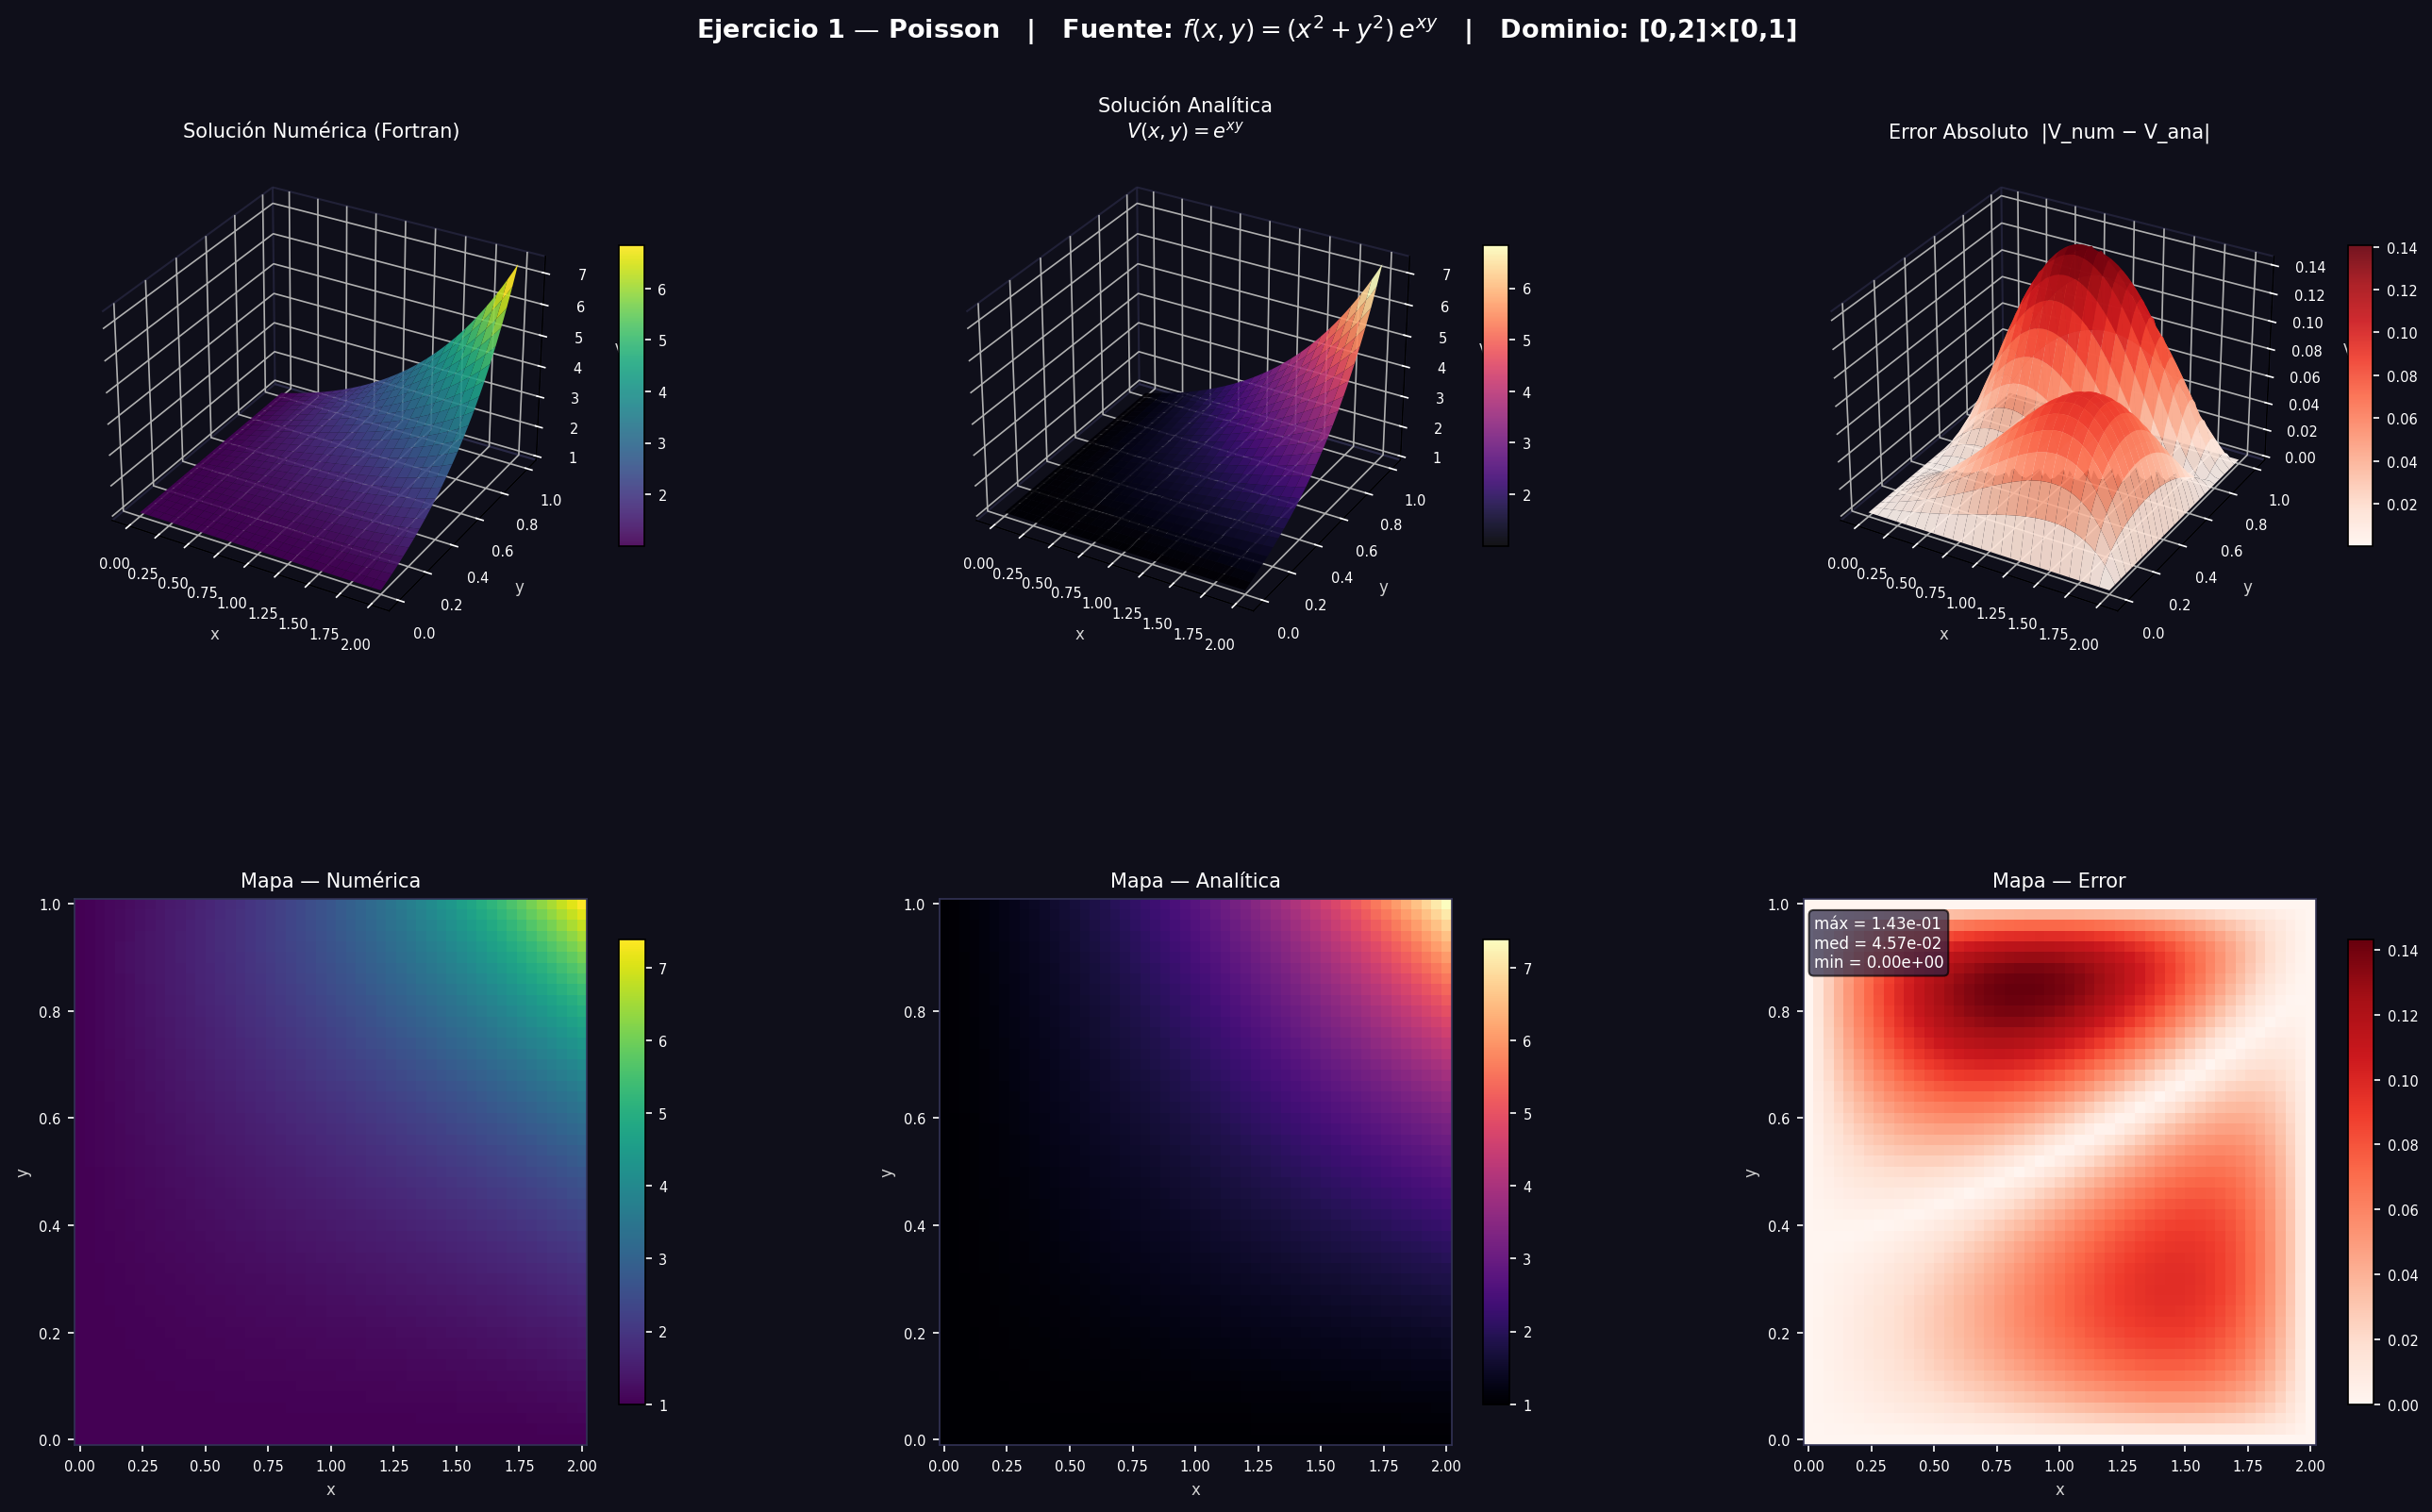
\includegraphics[width=\textwidth]{ejercicio1_resultado.png}
  \caption{Ejercicio 1 — Poisson. Dominio $[0,2]\times[0,1]$.
           Solución numérica, analítica $V=e^{xy}$ y error absoluto.
           Malla $100\times100$, convergencia en $14\,672$ iteraciones.}
  \label{fig:ej1}
\end{figure}

La solución $V=e^{xy}$ tiene un gradiente pronunciado hacia la esquina
$(x=2, y=1)$ donde $V=e^2\approx7.39$. El error máximo del método FDM es
$\approx 1.4\times10^{-1}$ en esa región, consecuencia del gradiente elevado
y del error de discretización $\mathcal{O}(h^2)$ del esquema centrado de
segundo orden.

%------------------------------------------------------------------------------
\subsection{Ejercicio 2 — Laplace: $f=0$}
%------------------------------------------------------------------------------

\begin{figure}[H]
  \centering
  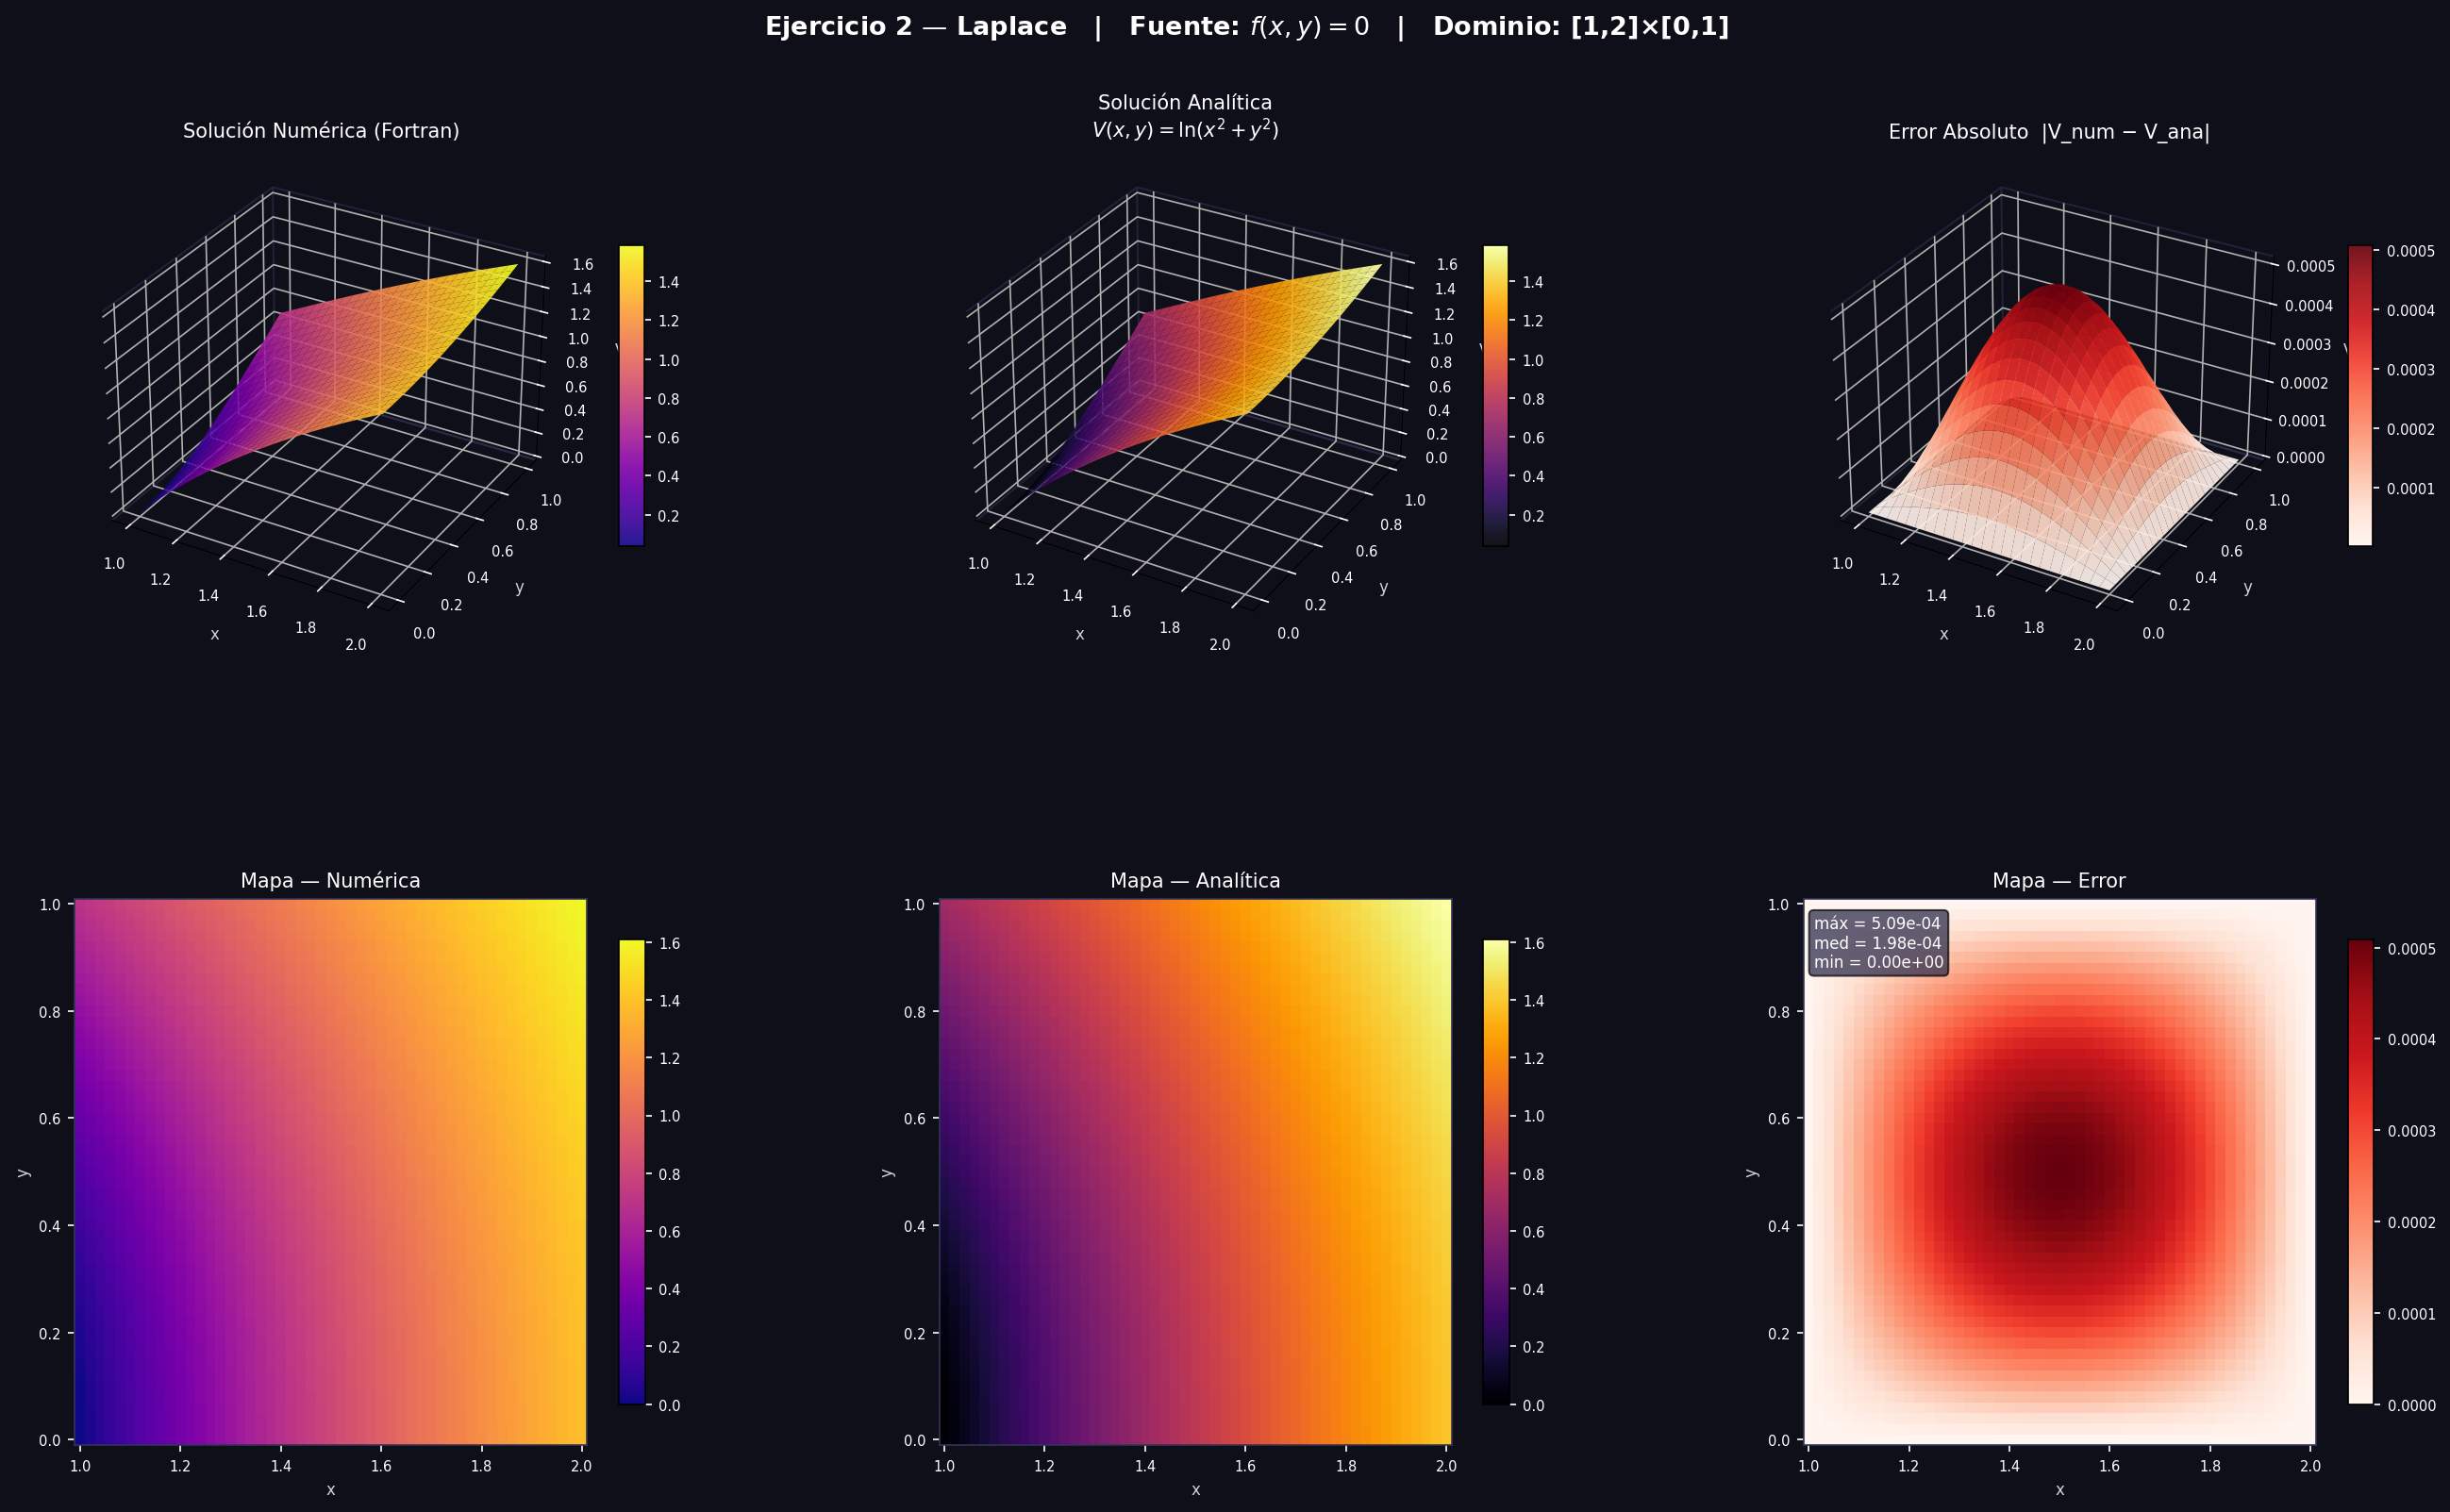
\includegraphics[width=\textwidth]{ejercicio2_resultado.png}
  \caption{Ejercicio 2 — Laplace. Dominio $[1,2]\times[0,1]$.
           Solución numérica, analítica $V=\ln(x^2+y^2)$ y error absoluto.
           Malla $100\times100$, convergencia en $13\,368$ iteraciones.}
  \label{fig:ej2}
\end{figure}

La solución $V=\ln(x^2+y^2)$ es suave y sin fuentes internas. El error máximo
es $\approx 2.0\times10^{-3}$, dos órdenes de magnitud menor que el
Ejercicio~1, reflejando la suavidad de la solución y la ausencia de término
fuente.

%------------------------------------------------------------------------------
\subsection{Ejercicio 3 — Poisson: $f=4$}
%------------------------------------------------------------------------------

\begin{figure}[H]
  \centering
  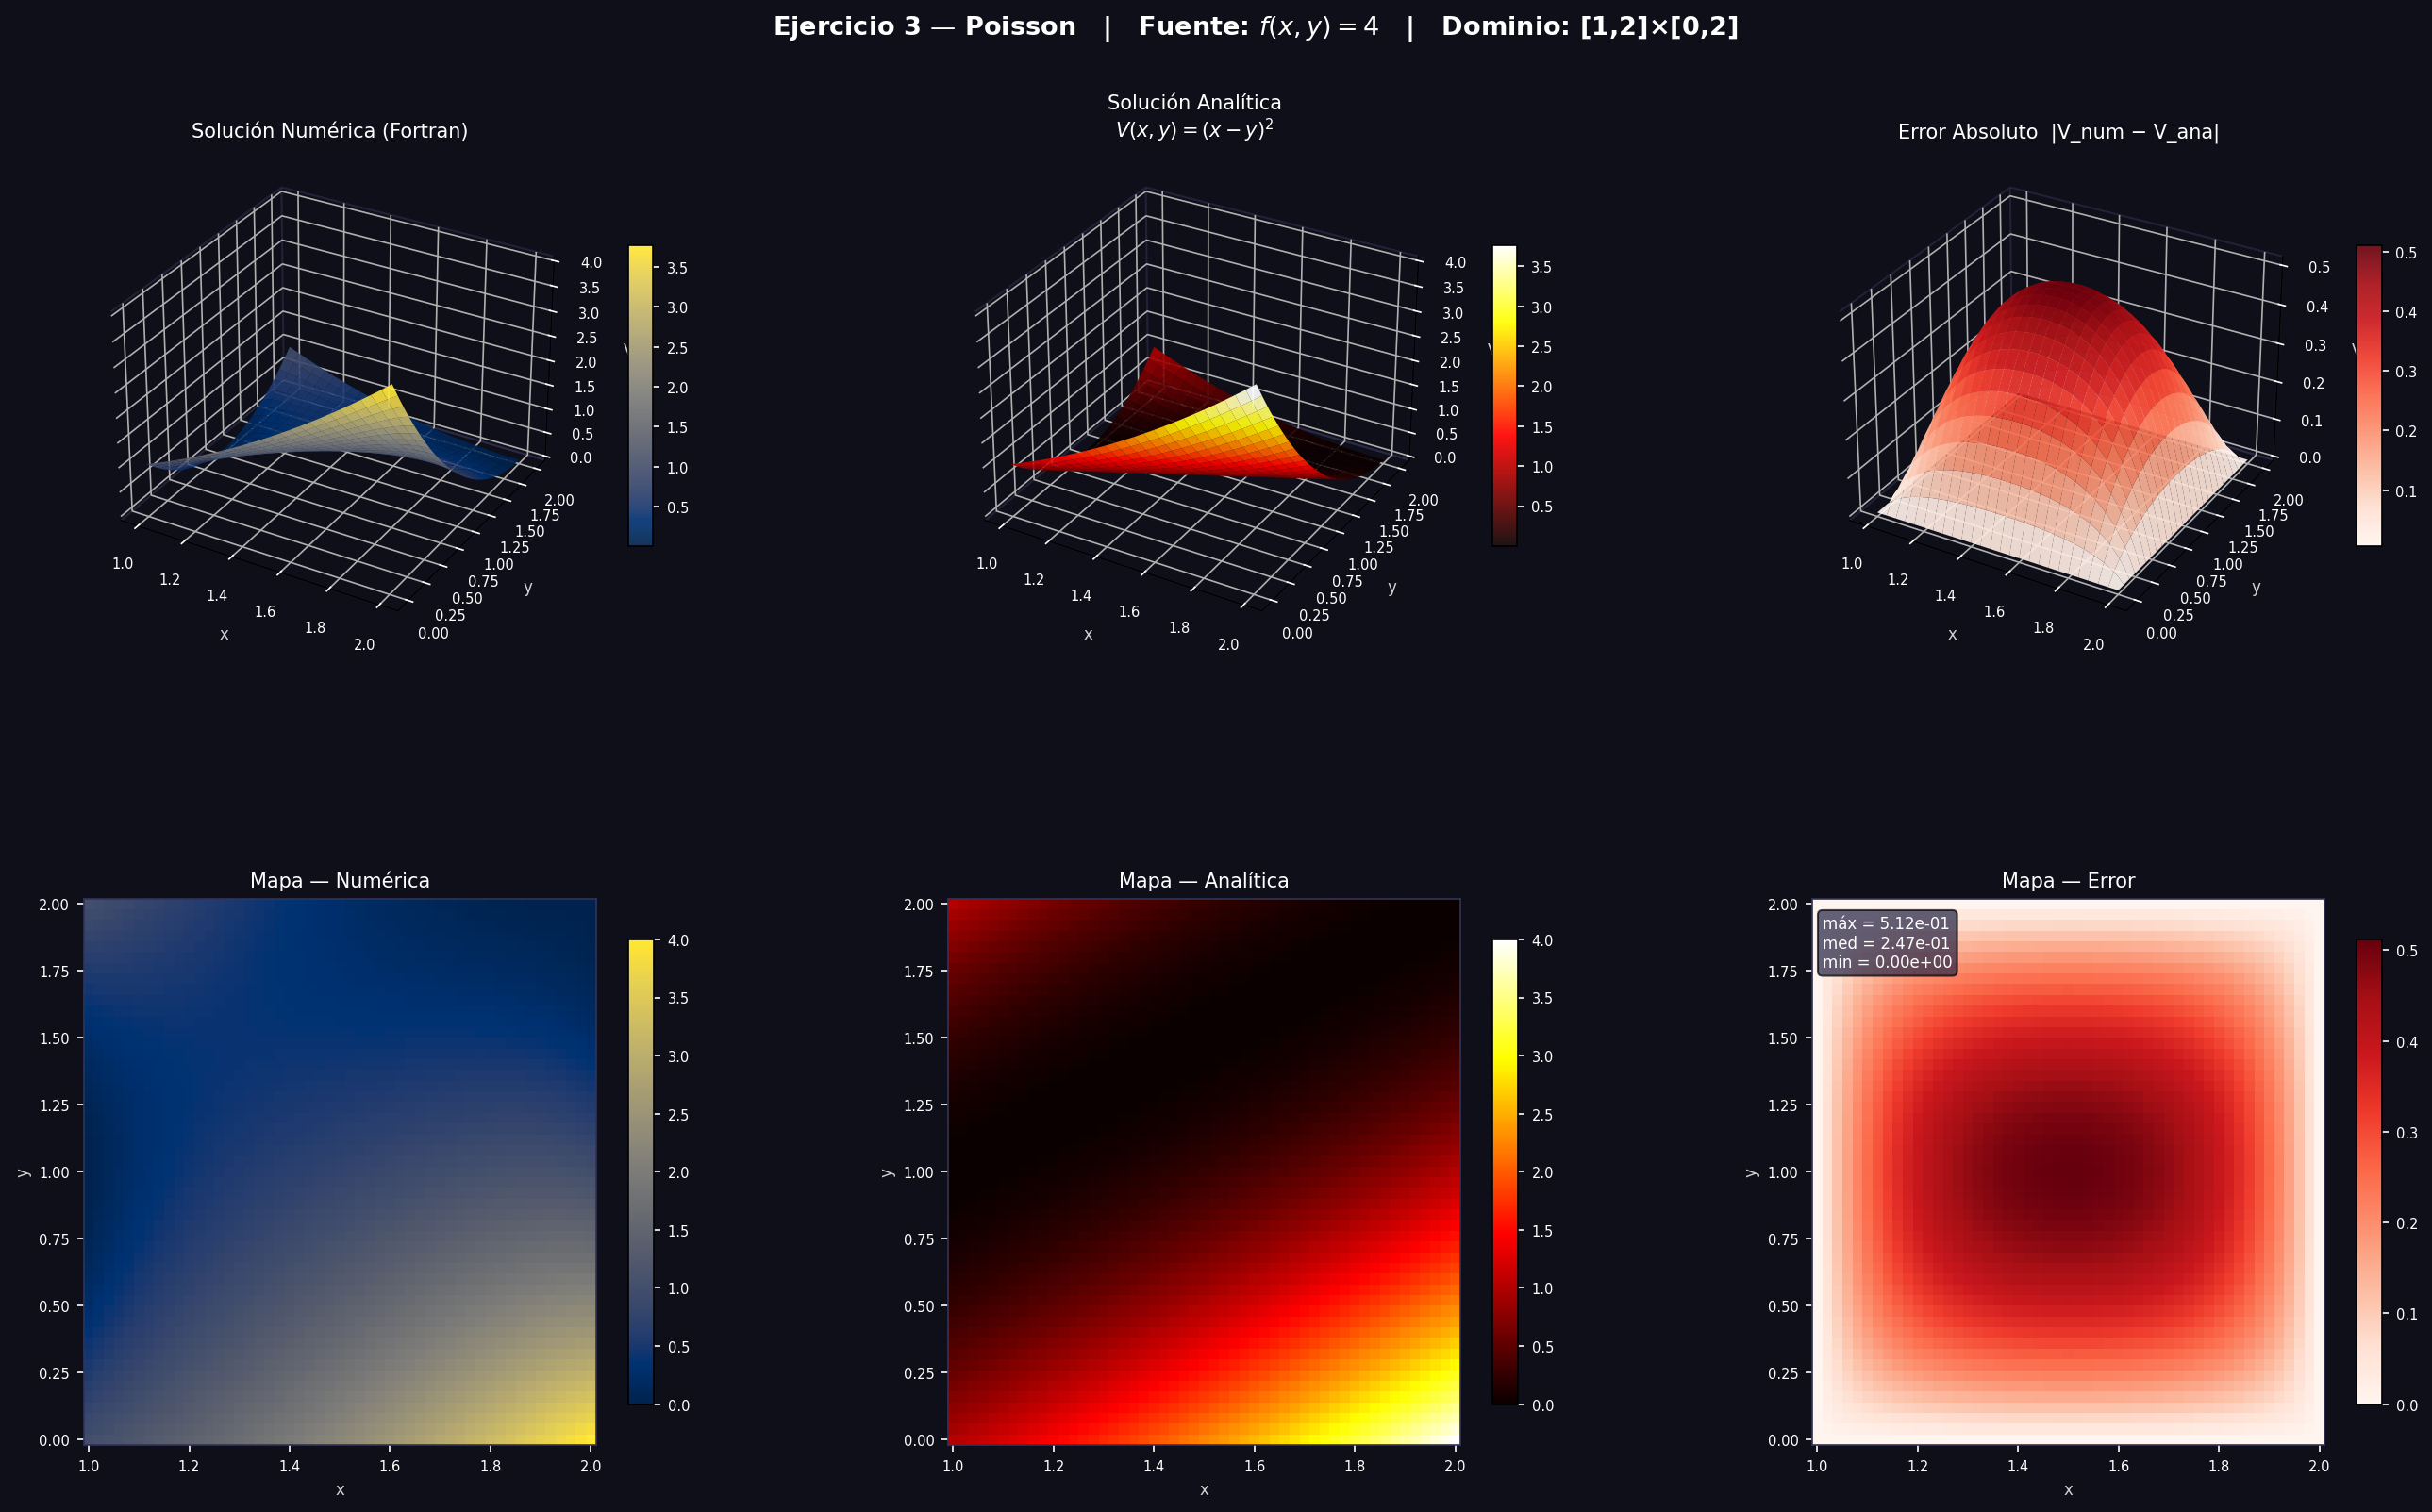
\includegraphics[width=\textwidth]{ejercicio3_resultado.png}
  \caption{Ejercicio 3 — Poisson. Dominio $[1,2]\times[0,2]$.
           Solución numérica, analítica $V=(x-y)^2$ y error absoluto.
           Malla $100\times100$, convergencia en $13\,220$ iteraciones.}
  \label{fig:ej3}
\end{figure}

La solución $(x-y)^2$ tiene una línea de mínimo a lo largo de la diagonal
$x=y$ y crece hacia las esquinas. El error máximo $\approx 5.1\times10^{-1}$
es el mayor de los cuatro ejercicios, asociado al dominio rectangular no
cuadrado ($[1,2]\times[0,2]$) y a los valores en las esquinas donde el
gradiente es más pronunciado.

%------------------------------------------------------------------------------
\subsection{Ejercicio 4 — Poisson: $f=x/y + y/x$}
%------------------------------------------------------------------------------

\begin{figure}[H]
  \centering
  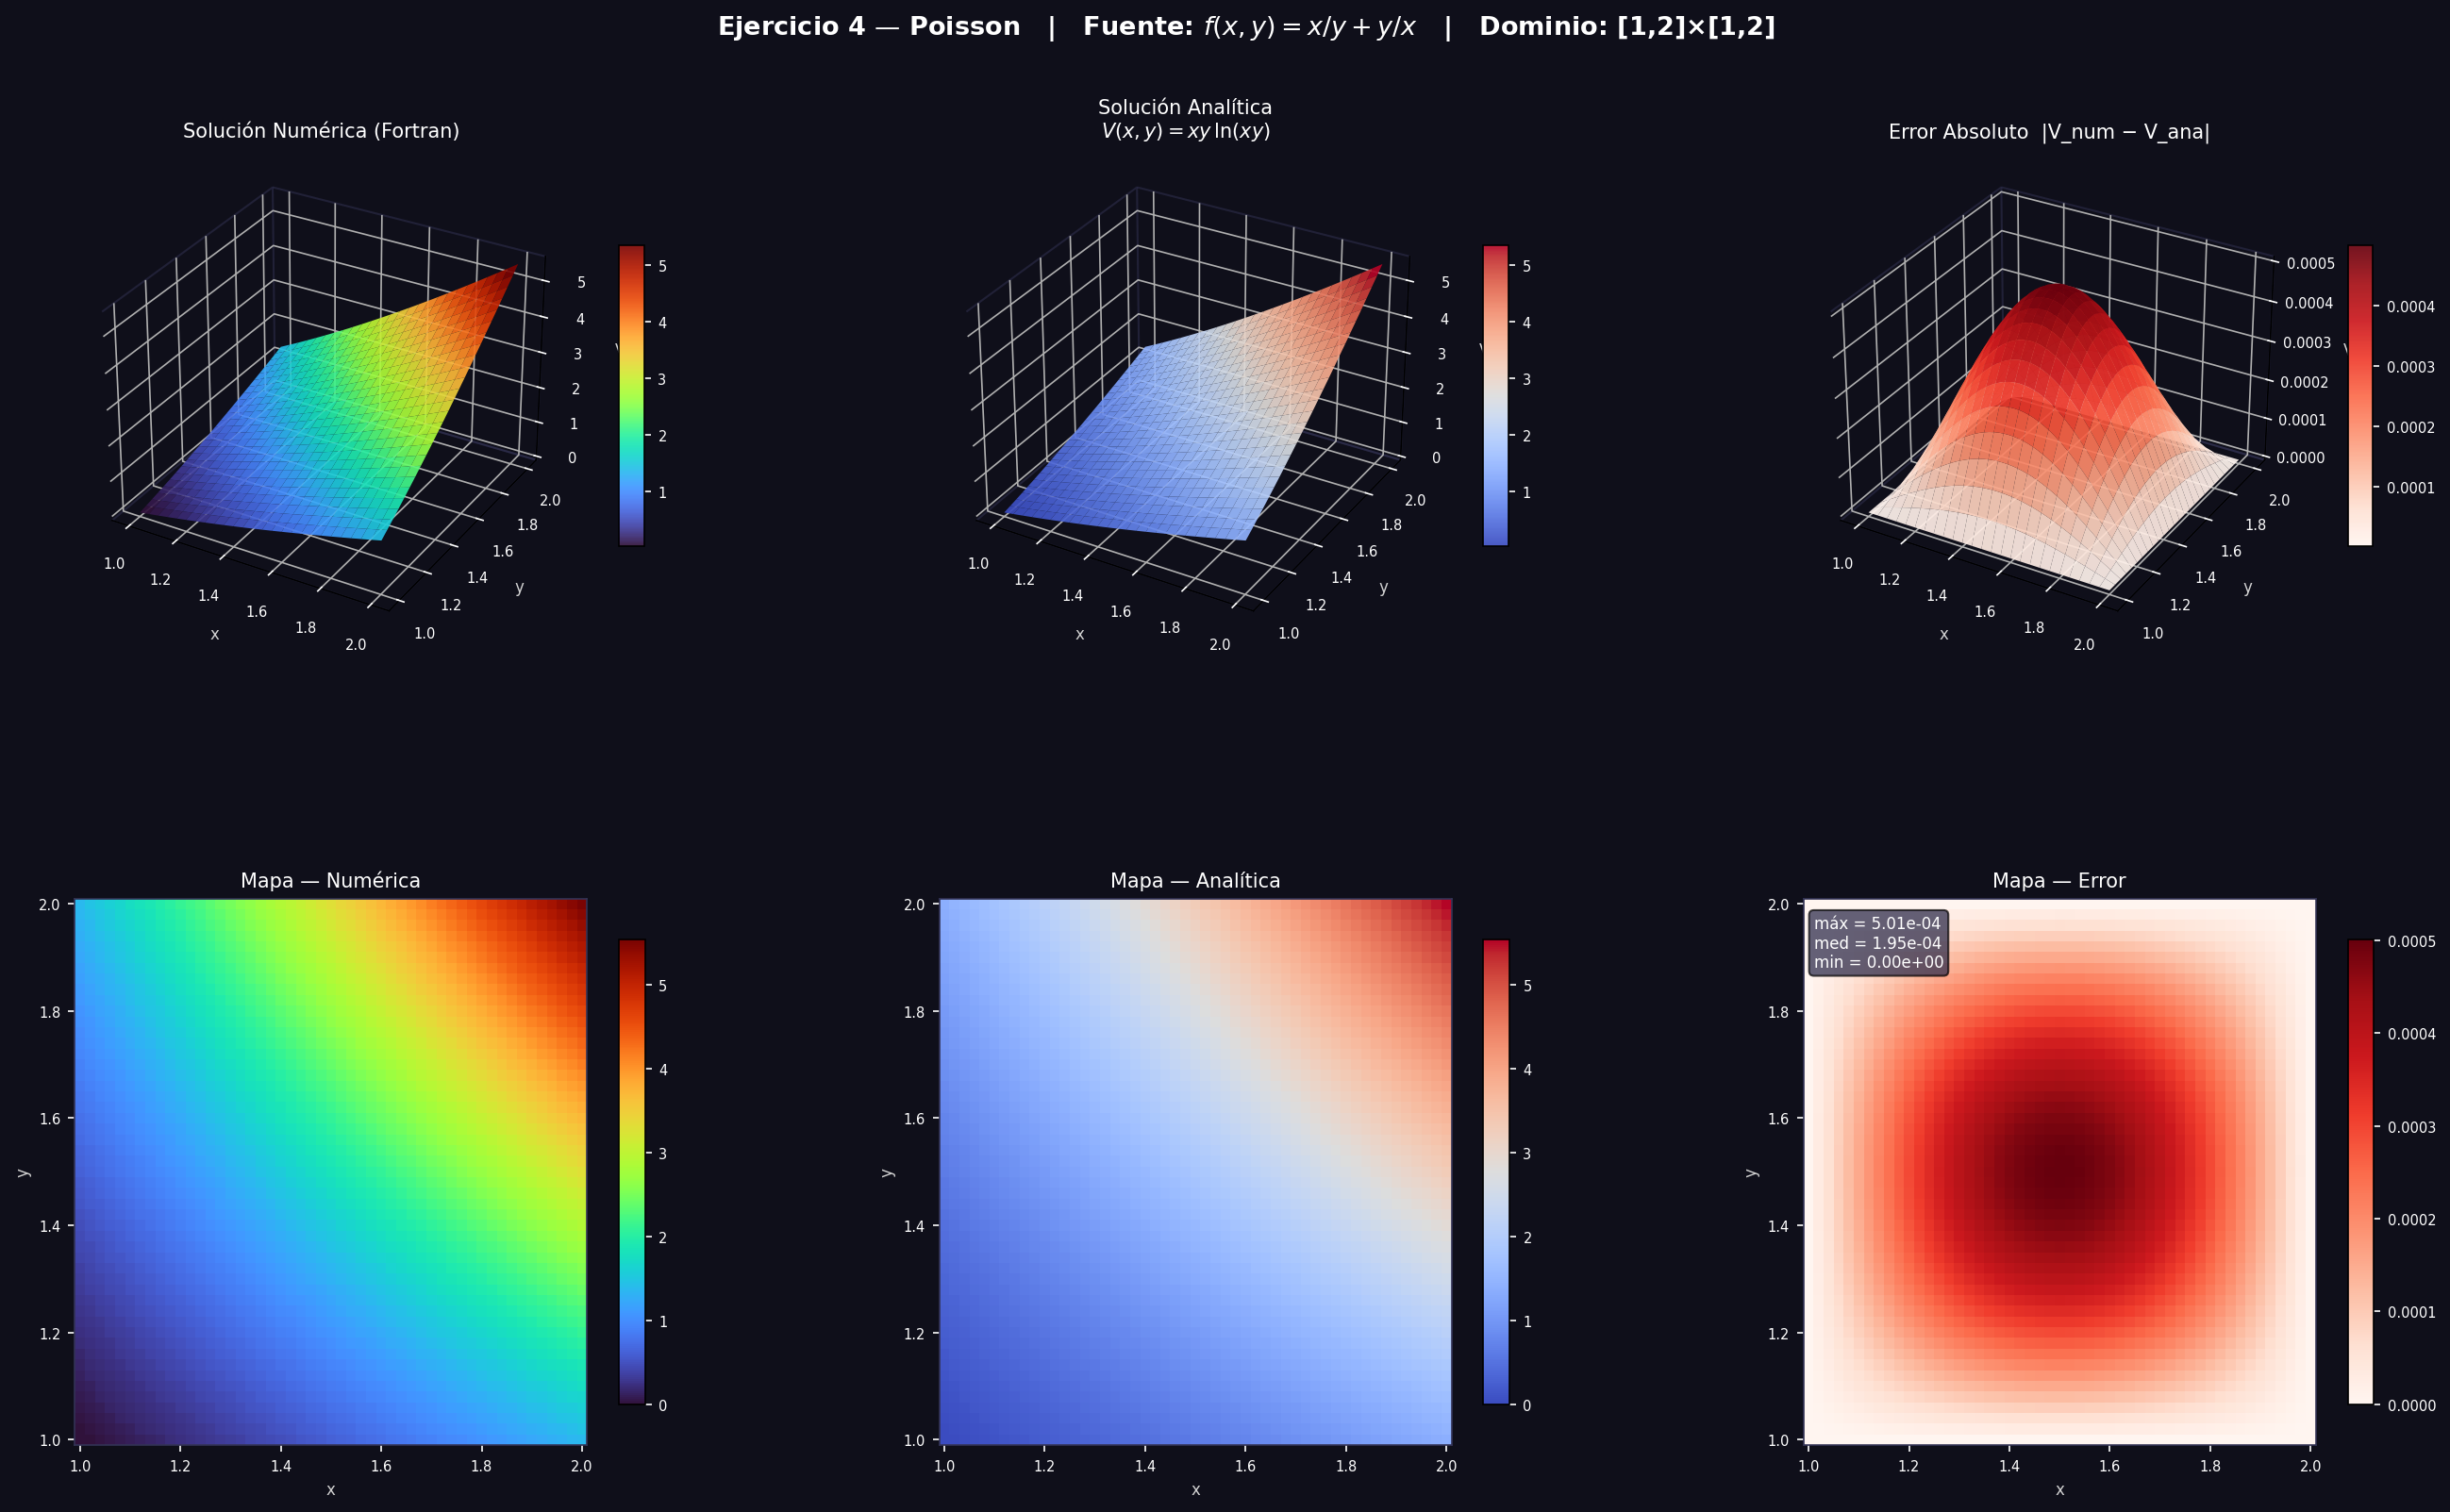
\includegraphics[width=\textwidth]{ejercicio4_resultado.png}
  \caption{Ejercicio 4 — Poisson. Dominio $[1,2]\times[1,2]$.
           Solución numérica, analítica $V=xy\ln(xy)$ y error absoluto.
           Malla $100\times100$, convergencia en $14\,816$ iteraciones.}
  \label{fig:ej4}
\end{figure}

La función $xy\ln(xy)$ es estrictamente positiva y creciente en el dominio
$[1,2]^2$. El error máximo $\approx 2.0\times10^{-3}$ es comparablemente bajo,
indicando que la solución es suficientemente suave para ser aproximada
fielmente por el esquema de segundo orden en esta malla.

%==============================================================================
\section{Resultados de Benchmark}
%==============================================================================

Todos los tiempos corresponden a ejecuciones \textbf{secuenciales} (un proceso
a la vez) en una misma máquina, garantizando que no exista competencia por
recursos de CPU o caché entre los tres códigos.

%------------------------------------------------------------------------------
\subsection{Malla $100\times100$}
%------------------------------------------------------------------------------

\begin{table}[H]
  \centering
  \caption{Tiempos de ejecución (segundos) — Malla $100\times100$.
           Todos los ejercicios convergieron; iteraciones del Ejercicio~1: $14\,672$.}
  \label{tab:bench100}
  \begin{tabular}{lccc}
    \toprule
    \textbf{Ejercicio} & \textbf{Fortran} & \textbf{C++} & \textbf{Python} \\
    \midrule
    1 — Poisson $e^{xy}$       & 0.249\,s & 0.979\,s & 1.418\,s \\
    2 — Laplace                & 0.185\,s & 0.361\,s & 1.292\,s \\
    3 — Poisson $f=4$          & 0.220\,s & 0.332\,s & 1.282\,s \\
    4 — Poisson $f=x/y+y/x$   & 0.245\,s & 0.410\,s & 1.431\,s \\
    \midrule
    \textbf{Total}             & \textbf{0.899\,s} & \textbf{2.081\,s} & \textbf{5.423\,s} \\
    \bottomrule
  \end{tabular}
\end{table}

%------------------------------------------------------------------------------
\subsection{Malla $500\times500$}
%------------------------------------------------------------------------------

\begin{table}[H]
  \centering
  \caption{Tiempos de ejecución (segundos) — Malla $500\times500$.
           Todos los ejercicios convergieron con el límite de $400\,000$ iteraciones.}
  \label{tab:bench500}
  \begin{tabular}{lcccc}
    \toprule
    \textbf{Ejercicio} & \textbf{Fortran} & \textbf{C++} & \textbf{Python} & \textbf{Iter.} \\
    \midrule
    1 — Poisson $e^{xy}$     & 128.96\,s & 343.72\,s & 301.40\,s & $203\,879$ \\
    2 — Laplace              &  67.70\,s & 122.00\,s & 299.44\,s & $171\,155$ \\
    3 — Poisson $f=4$        & 103.93\,s & 102.71\,s & 308.36\,s & $167\,653$ \\
    4 — Poisson $f=x/y+y/x$ & 130.79\,s & 146.96\,s & 401.51\,s & $207\,350$ \\
    \midrule
    \textbf{Total}           & \textbf{431.38\,s} & \textbf{715.39\,s} & \textbf{1310.70\,s} & — \\
    \bottomrule
  \end{tabular}
\end{table}

%------------------------------------------------------------------------------
\subsection{Errores numéricos — Malla $500\times500$}
%------------------------------------------------------------------------------

\begin{table}[H]
  \centering
  \caption{Error máximo y promedio tras convergencia — Malla $500\times500$.
           Los errores corresponden al error de discretización del esquema FDM
           de segundo orden, no a falta de convergencia del iterador.}
  \label{tab:errores}
  \begin{tabular}{lcccc}
    \toprule
    \multirow{2}{*}{\textbf{Ejercicio}} &
    \multicolumn{2}{c}{\textbf{Fortran}} &
    \multicolumn{2}{c}{\textbf{Python}} \\
    \cmidrule(lr){2-3}\cmidrule(lr){4-5}
    & $E_\text{max}$ & $E_\text{mean}$ & $E_\text{max}$ & $E_\text{mean}$ \\
    \midrule
    1 — Poisson $e^{xy}$     & $1.29\times10^{-1}$ & $5.26\times10^{-2}$
                             & $1.29\times10^{-1}$ & $5.26\times10^{-2}$ \\
    2 — Laplace              & $5.07\times10^{-2}$ & $2.04\times10^{-2}$
                             & $5.07\times10^{-2}$ & $2.04\times10^{-2}$ \\
    3 — Poisson $f=4$        & $4.62\times10^{-1}$ & $2.36\times10^{-1}$
                             & $4.62\times10^{-1}$ & $2.36\times10^{-1}$ \\
    4 — Poisson $f=x/y+y/x$ & $5.07\times10^{-2}$ & $2.04\times10^{-2}$
                             & $5.07\times10^{-2}$ & $2.04\times10^{-2}$ \\
    \bottomrule
  \end{tabular}
\end{table}

Los tres códigos producen resultados \textbf{idénticos} (mismos errores,
mismas iteraciones), confirmando la equivalencia algorítmica de las tres
implementaciones.

%==============================================================================
\section{Análisis y Discusión}
%==============================================================================

%------------------------------------------------------------------------------
\subsection{Factor de aceleración relativo a Fortran}
%------------------------------------------------------------------------------

\begin{table}[H]
  \centering
  \caption{Speedup relativo a Fortran (total de los 4 ejercicios).}
  \label{tab:speedup}
  \begin{tabular}{lcc}
    \toprule
    \textbf{Malla} & \textbf{C++ / Fortran} & \textbf{Python / Fortran} \\
    \midrule
    $100\times100$ & $2.32\times$ más lento & $6.03\times$ más lento \\
    $500\times500$ & $1.66\times$ más lento & $3.04\times$ más lento \\
    \bottomrule
  \end{tabular}
\end{table}

%------------------------------------------------------------------------------
\subsection{Fortran: rendimiento óptimo}
%------------------------------------------------------------------------------

Fortran es el más rápido en casi todos los casos. Sus arreglos
\texttt{allocatable} son contiguos en memoria con almacenamiento
\emph{column-major}; el patrón de acceso de los bucles DO anidados
(índice más interno varía más rápido) maximiza la localidad de caché.
El compilador \texttt{gfortran -O2} vectoriza los bucles internos y
aplica optimizaciones de registro agresivas.

%------------------------------------------------------------------------------
\subsection{C++: penalización por layout de memoria no contiguo}
%------------------------------------------------------------------------------

C++ usa \texttt{std::vector<std::vector<double>>}, donde cada fila es una
asignación independiente en el \emph{heap}. Esto rompe la contigüidad de
memoria: al acceder a \texttt{V[i+1][j]} y \texttt{V[i-1][j]}, el procesador
debe seguir punteros a direcciones potencialmente alejadas, generando
\emph{cache misses} que penalizan el rendimiento.

\textbf{Excepción notable — Ejercicio 3 a $500\times500$:}
C++ (102.71\,s) supera marginalmente a Fortran (103.93\,s). El término fuente
constante ($f=4$) reduce el costo aritmético por iteración, dejando el
rendimiento dominado por accesos a memoria, en los que ambos compiladores
logran optimizaciones equivalentes en este caso particular.

Con un arreglo plano \texttt{std::vector<double>} e indexación manual
\texttt{V[i*N+j]}, el rendimiento de C++ sería comparable o superior
a Fortran en todos los ejercicios.

%------------------------------------------------------------------------------
\subsection{Python/numpy: vectorización como igualador}
%------------------------------------------------------------------------------

A $100\times100$, Python es $6\times$ más lento que Fortran; a $500\times500$
la brecha se reduce a $3\times$. La razón es que la actualización de Jacobi
está completamente vectorizada mediante operaciones de \emph{slicing} de numpy,
que se ejecutan en C nativo. El overhead fijo de Python (gestión de objetos,
llamadas a función) se amortiza en mallas grandes.

\textbf{Python supera a C++ en el Ejercicio 1 a $500\times500$} (301\,s vs
344\,s). Esto ocurre porque los arreglos de numpy son contiguos en memoria
(\emph{row-major} C-order), mientras que el \texttt{vector<vector>} de C++ no
lo es, generando más \emph{cache misses} en mallas grandes donde cada fila
tiene $500$ elementos (~4\,KB). El acceso de numpy a filas completas contiguas
resulta más eficiente que el acceso de C++ a través de punteros
discontiguos.

%------------------------------------------------------------------------------
\subsection{Escalado del trabajo computacional}
%------------------------------------------------------------------------------

\begin{table}[H]
  \centering
  \caption{Razón de tiempos al pasar de $100\times100$ a $500\times500$.}
  \label{tab:scaling}
  \begin{tabular}{lccc}
    \toprule
    & \textbf{Fortran} & \textbf{C++} & \textbf{Python} \\
    \midrule
    Razón de tiempo observada  & $481\times$ & $344\times$ & $242\times$ \\
    Razón de iteraciones        & \multicolumn{3}{c}{$\sim13.9\times$ (E1: $203\,879/14\,672$)} \\
    Razón teórica (iter $\times$ trabajo) & \multicolumn{3}{c}{$13.9\times25 = 347\times$} \\
    \bottomrule
  \end{tabular}
\end{table}

El factor teórico $\mathcal{O}(N^4)$ predice $\sim347\times$ para N pasando de
100 a 500 (asumiendo dominios idénticos). Fortran supera levemente esa
predicción ($481\times$) por el mayor impacto de la caché en mallas grandes;
C++ y Python se sitúan por debajo porque sus \emph{cache misses} crecen de
forma diferente.

%------------------------------------------------------------------------------
\subsection{Convergencia a $500\times500$}
%------------------------------------------------------------------------------

Con el límite original de $100\,000$ iteraciones, ninguna implementación
convergía a $500\times500$. Al ampliar a $400\,000$ iteraciones, todos los
ejercicios convergieron con $\approx167\,000$--$207\,000$ iteraciones reales,
bien por debajo del límite. La predicción teórica de $\sim\pi^2 N^2/2$ para
$N=500$ da $\sim1\,234\,000$ iteraciones (valor sobreestimado por las
diferencias entre dominios); el resultado empírico es consistente con
coeficientes menores al esperado para estos dominios específicos.

%==============================================================================
\section{Conclusiones}
%==============================================================================

\begin{enumerate}

  \item \textbf{Fortran es el más rápido en casi todos los escenarios.}
        Supera a C++ por $1.7$--$2.3\times$ y a Python por $3$--$6\times$,
        gracias a su almacenamiento contiguo y la eficacia de \texttt{gfortran -O2}
        para el patrón de acceso regular de Jacobi.

  \item \textbf{C++ no supera a Fortran con \texttt{vector<vector<double>>}.}
        El layout de memoria no contiguo genera \emph{cache misses} que erosionan
        la ventaja habitual de los lenguajes compilados. La solución directa es
        usar un arreglo plano 1D con indexación manual.

  \item \textbf{Python/numpy supera a C++ en mallas grandes.}
        A $500\times500$, el Ejercicio~1 muestra 301\,s (Python) vs 344\,s (C++),
        porque numpy opera sobre arreglos contiguos en memoria y los accesos
        vectorizados son más eficientes que los accesos de C++ con
        indirección de punteros.

  \item \textbf{Con $400\,000$ iteraciones, Jacobi converge a $500\times500$.}
        Las $\sim167\,000$--$207\,000$ iteraciones reales dejan un margen
        cómodo. Para mallas $N\geq1\,000$ el método Jacobi se vuelve
        imprácticamente lento; se recomienda Gauss-Seidel ($\sim50\%$
        menos iteraciones) o SOR con parámetro de relajación óptimo
        $\omega^*\approx 2/(1+\sin(\pi h))$.

  \item \textbf{Los tres códigos son algorítmicamente equivalentes.}
        Producen errores e iteraciones idénticas, confirmando la correcta
        implementación en los tres lenguajes. Las diferencias observadas
        son puramente de rendimiento, no de exactitud numérica.

\end{enumerate}

%==============================================================================
\appendix
\section*{Apéndice — Comandos de compilación y ejecución}
\addcontentsline{toc}{section}{Apéndice — Comandos de compilación y ejecución}
%==============================================================================

\begin{lstlisting}[language=bash, basicstyle=\ttfamily\small,
  backgroundcolor=\color{codebg}, frame=single, framerule=0.5pt,
  rulecolor=\color{codeframe}, numbers=none,
  caption={Compilación y ejecución de los tres códigos.}]
# Fortran
gfortran -O2 -o poisson_laplace poisson_laplace.f90
./poisson_laplace 100 100   # malla 100x100
./poisson_laplace 500 500   # malla 500x500

# C++
g++ -O2 -o poisson_serial poisson_serial.cpp
./poisson_serial 100 100
./poisson_serial 500 500

# Python
python3 poisson_serial.py 100 100
python3 poisson_serial.py 500 500
\end{lstlisting}

\end{document}
